\documentclass[conference]{IEEEtran}
\usepackage[T1]{fontenc}
\usepackage{amsmath,amssymb}
\usepackage{graphicx}
\usepackage{booktabs}
\usepackage[hidelinks]{hyperref}
\graphicspath{{../figures/}}
\IfFileExists{numbers.tex}{% Generated by experiments/make_figures.py from results/. Do not edit by hand.
\newcommand{\brMPHeuqFive}{0.48}
\newcommand{\ciMPHeuqFive}{0.02}
\newcommand{\brMPHeuqSix}{0.28}
\newcommand{\ciMPHeuqSix}{0.02}
\newcommand{\brMPHeuqSeven}{0.10}
\newcommand{\ciMPHeuqSeven}{0.02}
\newcommand{\brMPHeuqEight}{0.02}
\newcommand{\ciMPHeuqEight}{0.01}
\newcommand{\brMPHeuqNine}{0.01}
\newcommand{\ciMPHeuqNine}{0.00}
\newcommand{\brMPHeuDoneqFive}{0.09}
\newcommand{\ciMPHeuDoneqFive}{0.02}
\newcommand{\brMPHeuDoneqSix}{0.03}
\newcommand{\ciMPHeuDoneqSix}{0.01}
\newcommand{\brMPHeuDoneqSeven}{0.01}
\newcommand{\ciMPHeuDoneqSeven}{0.00}
\newcommand{\brMPHeuDoneqEight}{0.00}
\newcommand{\ciMPHeuDoneqEight}{0.00}
\newcommand{\brMPHeuDoneqNine}{0.00}
\newcommand{\ciMPHeuDoneqNine}{0.00}
\newcommand{\brMPHeuDeadqFive}{0.25}
\newcommand{\ciMPHeuDeadqFive}{0.02}
\newcommand{\brMPHeuDeadqSix}{0.12}
\newcommand{\ciMPHeuDeadqSix}{0.01}
\newcommand{\brMPHeuDeadqSeven}{0.03}
\newcommand{\ciMPHeuDeadqSeven}{0.01}
\newcommand{\brMPHeuDeadqEight}{0.01}
\newcommand{\ciMPHeuDeadqEight}{0.00}
\newcommand{\brMPHeuDeadqNine}{0.00}
\newcommand{\ciMPHeuDeadqNine}{0.00}
\newcommand{\brMPILPqFive}{0.07}
\newcommand{\ciMPILPqFive}{0.02}
\newcommand{\brMPILPqSix}{0.03}
\newcommand{\ciMPILPqSix}{0.01}
\newcommand{\brMPILPqSeven}{0.01}
\newcommand{\ciMPILPqSeven}{0.01}
\newcommand{\brMPILPqEight}{0.00}
\newcommand{\ciMPILPqEight}{0.00}
\newcommand{\brMPILPqNine}{0.00}
\newcommand{\ciMPILPqNine}{0.00}
\newcommand{\brMPILPDeltaqFive}{0.18}
\newcommand{\ciMPILPDeltaqFive}{0.03}
\newcommand{\brMPILPDeltaqSix}{0.06}
\newcommand{\ciMPILPDeltaqSix}{0.02}
\newcommand{\brMPILPDeltaqSeven}{0.01}
\newcommand{\ciMPILPDeltaqSeven}{0.01}
\newcommand{\brMPILPDeltaqEight}{0.00}
\newcommand{\ciMPILPDeltaqEight}{0.00}
\newcommand{\brMPILPDeltaqNine}{0.00}
\newcommand{\ciMPILPDeltaqNine}{0.00}
\newcommand{\brSPHeuqFive}{0.69}
\newcommand{\ciSPHeuqFive}{0.02}
\newcommand{\brSPHeuqSix}{0.53}
\newcommand{\ciSPHeuqSix}{0.02}
\newcommand{\brSPHeuqSeven}{0.34}
\newcommand{\ciSPHeuqSeven}{0.03}
\newcommand{\brSPHeuqEight}{0.16}
\newcommand{\ciSPHeuqEight}{0.02}
\newcommand{\brSPHeuqNine}{0.04}
\newcommand{\ciSPHeuqNine}{0.01}
\newcommand{\brSPILPqFive}{0.11}
\newcommand{\ciSPILPqFive}{0.02}
\newcommand{\brSPILPqSix}{0.05}
\newcommand{\ciSPILPqSix}{0.01}
\newcommand{\brSPILPqSeven}{0.02}
\newcommand{\ciSPILPqSeven}{0.01}
\newcommand{\brSPILPqEight}{0.00}
\newcommand{\ciSPILPqEight}{0.00}
\newcommand{\brSPILPqNine}{0.00}
\newcommand{\ciSPILPqNine}{0.00}
\newcommand{\brSPSPFqFive}{0.68}
\newcommand{\ciSPSPFqFive}{0.02}
\newcommand{\brSPSPFqSix}{0.52}
\newcommand{\ciSPSPFqSix}{0.02}
\newcommand{\brSPSPFqSeven}{0.33}
\newcommand{\ciSPSPFqSeven}{0.03}
\newcommand{\brSPSPFqEight}{0.15}
\newcommand{\ciSPSPFqEight}{0.02}
\newcommand{\brSPSPFqNine}{0.04}
\newcommand{\ciSPSPFqNine}{0.01}
\newcommand{\gammaMPHeuqFive}{0.64}
\newcommand{\gammaciMPHeuqFive}{0.03}
\newcommand{\gammaMPHeuqSix}{0.60}
\newcommand{\gammaciMPHeuqSix}{0.02}
\newcommand{\gammaMPHeuqSeven}{0.49}
\newcommand{\gammaciMPHeuqSeven}{0.02}
\newcommand{\gammaMPHeuqEight}{0.42}
\newcommand{\gammaciMPHeuqEight}{0.02}
\newcommand{\gammaMPHeuqNine}{0.33}
\newcommand{\gammaciMPHeuqNine}{0.02}
\newcommand{\gammaMPHeuDoneqFive}{0.14}
\newcommand{\gammaciMPHeuDoneqFive}{0.01}
\newcommand{\gammaMPHeuDoneqSix}{0.12}
\newcommand{\gammaciMPHeuDoneqSix}{0.01}
\newcommand{\gammaMPHeuDoneqSeven}{0.09}
\newcommand{\gammaciMPHeuDoneqSeven}{0.01}
\newcommand{\gammaMPHeuDoneqEight}{0.07}
\newcommand{\gammaciMPHeuDoneqEight}{0.01}
\newcommand{\gammaMPHeuDoneqNine}{0.05}
\newcommand{\gammaciMPHeuDoneqNine}{0.01}
\newcommand{\gammaMPHeuDeadqFive}{0.17}
\newcommand{\gammaciMPHeuDeadqFive}{0.02}
\newcommand{\gammaMPHeuDeadqSix}{0.20}
\newcommand{\gammaciMPHeuDeadqSix}{0.03}
\newcommand{\gammaMPHeuDeadqSeven}{0.28}
\newcommand{\gammaciMPHeuDeadqSeven}{0.04}
\newcommand{\gammaMPHeuDeadqEight}{0.35}
\newcommand{\gammaciMPHeuDeadqEight}{0.02}
\newcommand{\gammaMPHeuDeadqNine}{0.31}
\newcommand{\gammaciMPHeuDeadqNine}{0.02}
\newcommand{\gammaMPILPqFive}{0.25}
\newcommand{\gammaciMPILPqFive}{0.02}
\newcommand{\gammaMPILPqSix}{0.22}
\newcommand{\gammaciMPILPqSix}{0.02}
\newcommand{\gammaMPILPqSeven}{0.19}
\newcommand{\gammaciMPILPqSeven}{0.01}
\newcommand{\gammaMPILPqEight}{0.20}
\newcommand{\gammaciMPILPqEight}{0.02}
\newcommand{\gammaMPILPqNine}{0.15}
\newcommand{\gammaciMPILPqNine}{0.02}
\newcommand{\gammaMPILPDeltaqFive}{0.65}
\newcommand{\gammaciMPILPDeltaqFive}{0.02}
\newcommand{\gammaMPILPDeltaqSix}{0.57}
\newcommand{\gammaciMPILPDeltaqSix}{0.03}
\newcommand{\gammaMPILPDeltaqSeven}{0.44}
\newcommand{\gammaciMPILPDeltaqSeven}{0.03}
\newcommand{\gammaMPILPDeltaqEight}{0.31}
\newcommand{\gammaciMPILPDeltaqEight}{0.02}
\newcommand{\gammaMPILPDeltaqNine}{0.18}
\newcommand{\gammaciMPILPDeltaqNine}{0.02}
\newcommand{\gammaSPHeuqFive}{0.00}
\newcommand{\gammaciSPHeuqFive}{0.00}
\newcommand{\gammaSPHeuqSix}{0.00}
\newcommand{\gammaciSPHeuqSix}{0.00}
\newcommand{\gammaSPHeuqSeven}{0.00}
\newcommand{\gammaciSPHeuqSeven}{0.00}
\newcommand{\gammaSPHeuqEight}{0.00}
\newcommand{\gammaciSPHeuqEight}{0.00}
\newcommand{\gammaSPHeuqNine}{0.00}
\newcommand{\gammaciSPHeuqNine}{0.00}
\newcommand{\gammaSPILPqFive}{0.00}
\newcommand{\gammaciSPILPqFive}{0.00}
\newcommand{\gammaSPILPqSix}{0.00}
\newcommand{\gammaciSPILPqSix}{0.00}
\newcommand{\gammaSPILPqSeven}{0.00}
\newcommand{\gammaciSPILPqSeven}{0.00}
\newcommand{\gammaSPILPqEight}{0.00}
\newcommand{\gammaciSPILPqEight}{0.00}
\newcommand{\gammaSPILPqNine}{0.00}
\newcommand{\gammaciSPILPqNine}{0.00}
\newcommand{\gammaSPSPFqFive}{0.00}
\newcommand{\gammaciSPSPFqFive}{0.00}
\newcommand{\gammaSPSPFqSix}{0.00}
\newcommand{\gammaciSPSPFqSix}{0.00}
\newcommand{\gammaSPSPFqSeven}{0.00}
\newcommand{\gammaciSPSPFqSeven}{0.00}
\newcommand{\gammaSPSPFqEight}{0.00}
\newcommand{\gammaciSPSPFqEight}{0.00}
\newcommand{\gammaSPSPFqNine}{0.00}
\newcommand{\gammaciSPSPFqNine}{0.00}
\newcommand{\runtimeMPHeuqFive}{0.0}
\newcommand{\runtimeMPHeuqSix}{0.0}
\newcommand{\runtimeMPHeuqSeven}{0.0}
\newcommand{\runtimeMPHeuqEight}{0.0}
\newcommand{\runtimeMPHeuqNine}{0.0}
\newcommand{\runtimeMPHeuDoneqFive}{0.0}
\newcommand{\runtimeMPHeuDoneqSix}{0.0}
\newcommand{\runtimeMPHeuDoneqSeven}{0.0}
\newcommand{\runtimeMPHeuDoneqEight}{0.0}
\newcommand{\runtimeMPHeuDoneqNine}{0.0}
\newcommand{\runtimeMPHeuDeadqFive}{0.0}
\newcommand{\runtimeMPHeuDeadqSix}{0.0}
\newcommand{\runtimeMPHeuDeadqSeven}{0.0}
\newcommand{\runtimeMPHeuDeadqEight}{0.0}
\newcommand{\runtimeMPHeuDeadqNine}{0.0}
\newcommand{\runtimeMPILPqFive}{1.2}
\newcommand{\runtimeMPILPqSix}{1.3}
\newcommand{\runtimeMPILPqSeven}{1.3}
\newcommand{\runtimeMPILPqEight}{1.4}
\newcommand{\runtimeMPILPqNine}{1.4}
\newcommand{\runtimeMPILPDeltaqFive}{0.4}
\newcommand{\runtimeMPILPDeltaqSix}{0.9}
\newcommand{\runtimeMPILPDeltaqSeven}{1.3}
\newcommand{\runtimeMPILPDeltaqEight}{2.3}
\newcommand{\runtimeMPILPDeltaqNine}{2.3}
\newcommand{\runtimeSPHeuqFive}{0.0}
\newcommand{\runtimeSPHeuqSix}{0.0}
\newcommand{\runtimeSPHeuqSeven}{0.0}
\newcommand{\runtimeSPHeuqEight}{0.0}
\newcommand{\runtimeSPHeuqNine}{0.0}
\newcommand{\runtimeSPILPqFive}{0.1}
\newcommand{\runtimeSPILPqSix}{0.1}
\newcommand{\runtimeSPILPqSeven}{0.1}
\newcommand{\runtimeSPILPqEight}{0.1}
\newcommand{\runtimeSPILPqNine}{0.1}
\newcommand{\runtimeSPSPFqFive}{0.0}
\newcommand{\runtimeSPSPFqSix}{0.0}
\newcommand{\runtimeSPSPFqSeven}{0.0}
\newcommand{\runtimeSPSPFqEight}{0.0}
\newcommand{\runtimeSPSPFqNine}{0.0}
\newcommand{\brMPHeuRTwenty}{0.00}
\newcommand{\ciMPHeuRTwenty}{0.01}
\newcommand{\brMPHeuRForty}{0.02}
\newcommand{\ciMPHeuRForty}{0.01}
\newcommand{\brMPHeuRSixty}{0.10}
\newcommand{\ciMPHeuRSixty}{0.02}
\newcommand{\brMPHeuREighty}{0.24}
\newcommand{\ciMPHeuREighty}{0.02}
\newcommand{\brMPHeuRHundred}{0.37}
\newcommand{\ciMPHeuRHundred}{0.01}
\newcommand{\brMPILPRTwenty}{0.00}
\newcommand{\ciMPILPRTwenty}{0.00}
\newcommand{\brMPILPRForty}{0.00}
\newcommand{\ciMPILPRForty}{0.00}
\newcommand{\brMPILPRSixty}{0.01}
\newcommand{\ciMPILPRSixty}{0.01}
\newcommand{\brMPILPREighty}{0.04}
\newcommand{\ciMPILPREighty}{0.01}
\newcommand{\brMPILPRHundred}{0.09}
\newcommand{\ciMPILPRHundred}{0.01}
\newcommand{\brSPHeuRTwenty}{0.07}
\newcommand{\ciSPHeuRTwenty}{0.03}
\newcommand{\brSPHeuRForty}{0.20}
\newcommand{\ciSPHeuRForty}{0.03}
\newcommand{\brSPHeuRSixty}{0.34}
\newcommand{\ciSPHeuRSixty}{0.03}
\newcommand{\brSPHeuREighty}{0.44}
\newcommand{\ciSPHeuREighty}{0.02}
\newcommand{\brSPHeuRHundred}{0.52}
\newcommand{\ciSPHeuRHundred}{0.02}
\newcommand{\brSPILPRTwenty}{0.00}
\newcommand{\ciSPILPRTwenty}{0.00}
\newcommand{\brSPILPRForty}{0.00}
\newcommand{\ciSPILPRForty}{0.00}
\newcommand{\brSPILPRSixty}{0.02}
\newcommand{\ciSPILPRSixty}{0.01}
\newcommand{\brSPILPREighty}{0.06}
\newcommand{\ciSPILPREighty}{0.01}
\newcommand{\brSPILPRHundred}{0.11}
\newcommand{\ciSPILPRHundred}{0.01}
\newcommand{\brSPSPFRTwenty}{0.08}
\newcommand{\ciSPSPFRTwenty}{0.03}
\newcommand{\brSPSPFRForty}{0.20}
\newcommand{\ciSPSPFRForty}{0.03}
\newcommand{\brSPSPFRSixty}{0.33}
\newcommand{\ciSPSPFRSixty}{0.03}
\newcommand{\brSPSPFREighty}{0.43}
\newcommand{\ciSPSPFREighty}{0.02}
\newcommand{\brSPSPFRHundred}{0.51}
\newcommand{\ciSPSPFRHundred}{0.02}
\newcommand{\gammaMPHeuRTwenty}{0.50}
\newcommand{\gammaciMPHeuRTwenty}{0.03}
\newcommand{\gammaMPHeuRForty}{0.50}
\newcommand{\gammaciMPHeuRForty}{0.03}
\newcommand{\gammaMPHeuRSixty}{0.49}
\newcommand{\gammaciMPHeuRSixty}{0.02}
\newcommand{\gammaMPHeuREighty}{0.49}
\newcommand{\gammaciMPHeuREighty}{0.02}
\newcommand{\gammaMPHeuRHundred}{0.48}
\newcommand{\gammaciMPHeuRHundred}{0.02}
\newcommand{\gammaMPILPRTwenty}{0.26}
\newcommand{\gammaciMPILPRTwenty}{0.04}
\newcommand{\gammaMPILPRForty}{0.21}
\newcommand{\gammaciMPILPRForty}{0.02}
\newcommand{\gammaMPILPRSixty}{0.19}
\newcommand{\gammaciMPILPRSixty}{0.01}
\newcommand{\gammaMPILPREighty}{0.18}
\newcommand{\gammaciMPILPREighty}{0.02}
\newcommand{\gammaMPILPRHundred}{0.17}
\newcommand{\gammaciMPILPRHundred}{0.01}
\newcommand{\gammaSPHeuRTwenty}{0.00}
\newcommand{\gammaciSPHeuRTwenty}{0.00}
\newcommand{\gammaSPHeuRForty}{0.00}
\newcommand{\gammaciSPHeuRForty}{0.00}
\newcommand{\gammaSPHeuRSixty}{0.00}
\newcommand{\gammaciSPHeuRSixty}{0.00}
\newcommand{\gammaSPHeuREighty}{0.00}
\newcommand{\gammaciSPHeuREighty}{0.00}
\newcommand{\gammaSPHeuRHundred}{0.00}
\newcommand{\gammaciSPHeuRHundred}{0.00}
\newcommand{\gammaSPILPRTwenty}{0.00}
\newcommand{\gammaciSPILPRTwenty}{0.00}
\newcommand{\gammaSPILPRForty}{0.00}
\newcommand{\gammaciSPILPRForty}{0.00}
\newcommand{\gammaSPILPRSixty}{0.00}
\newcommand{\gammaciSPILPRSixty}{0.00}
\newcommand{\gammaSPILPREighty}{0.00}
\newcommand{\gammaciSPILPREighty}{0.00}
\newcommand{\gammaSPILPRHundred}{0.00}
\newcommand{\gammaciSPILPRHundred}{0.00}
\newcommand{\gammaSPSPFRTwenty}{0.00}
\newcommand{\gammaciSPSPFRTwenty}{0.00}
\newcommand{\gammaSPSPFRForty}{0.00}
\newcommand{\gammaciSPSPFRForty}{0.00}
\newcommand{\gammaSPSPFRSixty}{0.00}
\newcommand{\gammaciSPSPFRSixty}{0.00}
\newcommand{\gammaSPSPFREighty}{0.00}
\newcommand{\gammaciSPSPFREighty}{0.00}
\newcommand{\gammaSPSPFRHundred}{0.00}
\newcommand{\gammaciSPSPFRHundred}{0.00}
\newcommand{\runtimeMPHeuRTwenty}{0.0}
\newcommand{\runtimeMPHeuRForty}{0.0}
\newcommand{\runtimeMPHeuRSixty}{0.0}
\newcommand{\runtimeMPHeuREighty}{0.0}
\newcommand{\runtimeMPHeuRHundred}{0.1}
\newcommand{\runtimeMPILPRTwenty}{0.2}
\newcommand{\runtimeMPILPRForty}{0.6}
\newcommand{\runtimeMPILPRSixty}{1.3}
\newcommand{\runtimeMPILPREighty}{2.5}
\newcommand{\runtimeMPILPRHundred}{4.4}
\newcommand{\runtimeSPHeuRTwenty}{0.0}
\newcommand{\runtimeSPHeuRForty}{0.0}
\newcommand{\runtimeSPHeuRSixty}{0.0}
\newcommand{\runtimeSPHeuREighty}{0.0}
\newcommand{\runtimeSPHeuRHundred}{0.1}
\newcommand{\runtimeSPILPRTwenty}{0.0}
\newcommand{\runtimeSPILPRForty}{0.1}
\newcommand{\runtimeSPILPRSixty}{0.1}
\newcommand{\runtimeSPILPREighty}{0.1}
\newcommand{\runtimeSPILPRHundred}{0.2}
\newcommand{\runtimeSPSPFRTwenty}{0.0}
\newcommand{\runtimeSPSPFRForty}{0.0}
\newcommand{\runtimeSPSPFRSixty}{0.0}
\newcommand{\runtimeSPSPFREighty}{0.0}
\newcommand{\runtimeSPSPFRHundred}{0.0}
\newcommand{\nChoice}{\ensuremath{\mathcal{U}\{2,2\}}}
\newcommand{\nChoiceLo}{2}
\newcommand{\nChoiceHi}{2}
\newcommand{\gammaRMSE}{0.077}
\newcommand{\rmseOneOne}{0.567}
\newcommand{\rmseOneTwo}{0.328}
\newcommand{\rmseOneThree}{0.163}
\newcommand{\rmseOneFour}{0.146}
\newcommand{\rmseOneFive}{0.146}
\newcommand{\rmseOneSix}{0.145}
\newcommand{\rmseTwoTwo}{0.077}
\newcommand{\rmseTwoThree}{0.155}
\newcommand{\rmseTwoFour}{0.235}
\newcommand{\rmseTwoFive}{0.260}
\newcommand{\rmseTwoSix}{0.282}
\newcommand{\rmseThreeThree}{0.368}
\newcommand{\rmseThreeFour}{0.393}
\newcommand{\rmseThreeFive}{0.400}
\newcommand{\rmseThreeSix}{0.409}
\newcommand{\rmseTwoTen}{0.298}
\newcommand{\paperBRMPILPqNine}{0.27}
\newcommand{\paperBRSPILPqNine}{0.42}
\newcommand{\paperGammaMPILPqFive}{0.70}
\newcommand{\paperGammaMPILPqSix}{0.68}
\newcommand{\paperGammaMPILPqSeven}{0.64}
\newcommand{\paperGammaMPILPqEight}{0.58}
\newcommand{\paperGammaMPILPqNine}{0.52}
\newcommand{\paperGammaMPHeuqFive}{0.66}
\newcommand{\paperGammaMPHeuqSix}{0.62}
\newcommand{\paperGammaMPHeuqSeven}{0.57}
\newcommand{\paperGammaMPHeuqEight}{0.51}
\newcommand{\paperGammaMPHeuqNine}{0.45}
\newcommand{\paperTimeSPILPqFive}{428}
\newcommand{\paperTimeSPILPqSix}{413}
\newcommand{\paperTimeSPILPqSeven}{396}
\newcommand{\paperTimeSPILPqEight}{382}
\newcommand{\paperTimeSPILPqNine}{373}
\newcommand{\paperTimeMPILPqFive}{873}
\newcommand{\paperTimeMPILPqSix}{852}
\newcommand{\paperTimeMPILPqSeven}{838}
\newcommand{\paperTimeMPILPqEight}{806}
\newcommand{\paperTimeMPILPqNine}{783}
\newcommand{\paperTimeSPHeu}{1.4}
\newcommand{\paperTimeMPHeu}{2}
\newcommand{\paperBRLargeSPHeutcTenqNine}{0.231}
\newcommand{\paperBRLargeMPHeutcTenqNine}{0.156}
\newcommand{\paperBRLargeSPHeutcTwentyqNine}{0.254}
\newcommand{\paperBRLargeMPHeutcTwentyqNine}{0.173}
\newcommand{\auditWindows}{1372}
\newcommand{\auditViolations}{0}
\newcommand{\auditInconclusive}{0}
\newcommand{\ilpTimeLimitWindows}{0}
\newcommand{\ilpRuns}{750}
\newcommand{\extThreshold}{0.03}
\newcommand{\extDiffqFive}{0.23}
\newcommand{\extCIqFive}{0.02}
\newcommand{\extCIloqFive}{0.21}
\newcommand{\extCIhiqFive}{0.24}
\newcommand{\extDoneDiffqFive}{0.39}
\newcommand{\extDoneCIqFive}{0.01}
\newcommand{\extGapDeadqFive}{0.56}
\newcommand{\extGapDoneqFive}{0.96}
\newcommand{\extDiffqSix}{0.16}
\newcommand{\extCIqSix}{0.02}
\newcommand{\extCIloqSix}{0.14}
\newcommand{\extCIhiqSix}{0.18}
\newcommand{\extDoneDiffqSix}{0.25}
\newcommand{\extDoneCIqSix}{0.02}
\newcommand{\extGapDeadqSix}{0.65}
\newcommand{\extGapDoneqSix}{1.01}
\newcommand{\extDiffqSeven}{0.07}
\newcommand{\extCIqSeven}{0.02}
\newcommand{\extCIloqSeven}{0.05}
\newcommand{\extCIhiqSeven}{0.09}
\newcommand{\extDoneDiffqSeven}{0.10}
\newcommand{\extDoneCIqSeven}{0.02}
\newcommand{\extGapDeadqSeven}{0.73}
\newcommand{\extGapDoneqSeven}{1.00}
\newcommand{\extDiffqEight}{0.02}
\newcommand{\extCIqEight}{0.01}
\newcommand{\extCIloqEight}{0.01}
\newcommand{\extCIhiqEight}{0.03}
\newcommand{\extDoneDiffqEight}{0.02}
\newcommand{\extDoneCIqEight}{0.01}
\newcommand{\extGapDeadqEight}{0.86}
\newcommand{\extGapDoneqEight}{1.00}
\newcommand{\extDiffqNine}{0.01}
\newcommand{\extCIqNine}{0.00}
\newcommand{\extCIloqNine}{0.00}
\newcommand{\extCIhiqNine}{0.01}
\newcommand{\extDoneDiffqNine}{0.01}
\newcommand{\extDoneCIqNine}{0.00}
\newcommand{\extGapDeadqNine}{1.00}
\newcommand{\extGapDoneqNine}{1.00}
\newcommand{\extVerdict}{supported}
}{}
\IfFileExists{sensitivity.tex}{% Generated by experiments/sensitivity.py. Do not edit.
\newcommand{\sensBRBaseMPHeuqFive}{0.48}
\newcommand{\sensCIBaseMPHeuqFive}{0.02}
\newcommand{\sensBRBaseMPHeuqNine}{0.01}
\newcommand{\sensCIBaseMPHeuqNine}{0.00}
\newcommand{\sensBRBaseMPILPqFive}{0.07}
\newcommand{\sensCIBaseMPILPqFive}{0.02}
\newcommand{\sensBRBaseMPILPqNine}{0.00}
\newcommand{\sensCIBaseMPILPqNine}{0.00}
\newcommand{\sensBRBaseSPHeuqFive}{0.69}
\newcommand{\sensCIBaseSPHeuqFive}{0.02}
\newcommand{\sensBRBaseSPHeuqNine}{0.04}
\newcommand{\sensCIBaseSPHeuqNine}{0.01}
\newcommand{\sensBRBaseSPILPqFive}{0.12}
\newcommand{\sensCIBaseSPILPqFive}{0.02}
\newcommand{\sensBRBaseSPILPqNine}{0.00}
\newcommand{\sensCIBaseSPILPqNine}{0.00}
\newcommand{\sensBRGapsMPHeuqFive}{0.59}
\newcommand{\sensCIGapsMPHeuqFive}{0.02}
\newcommand{\sensBRGapsMPHeuqNine}{0.35}
\newcommand{\sensCIGapsMPHeuqNine}{0.03}
\newcommand{\sensBRGapsMPILPqFive}{0.37}
\newcommand{\sensCIGapsMPILPqFive}{0.02}
\newcommand{\sensBRGapsMPILPqNine}{0.35}
\newcommand{\sensCIGapsMPILPqNine}{0.03}
\newcommand{\sensBRGapsSPHeuqFive}{0.79}
\newcommand{\sensCIGapsSPHeuqFive}{0.02}
\newcommand{\sensBRGapsSPHeuqNine}{0.37}
\newcommand{\sensCIGapsSPHeuqNine}{0.02}
\newcommand{\sensBRGapsSPILPqFive}{0.39}
\newcommand{\sensCIGapsSPILPqFive}{0.02}
\newcommand{\sensBRGapsSPILPqNine}{0.35}
\newcommand{\sensCIGapsSPILPqNine}{0.03}
\newcommand{\sensBRGapsPerSlotMPHeuqFive}{0.85}
\newcommand{\sensCIGapsPerSlotMPHeuqFive}{0.01}
\newcommand{\sensBRGapsPerSlotMPHeuqNine}{0.65}
\newcommand{\sensCIGapsPerSlotMPHeuqNine}{0.02}
\newcommand{\sensBRGapsPerSlotMPILPqFive}{0.63}
\newcommand{\sensCIGapsPerSlotMPILPqFive}{0.02}
\newcommand{\sensBRGapsPerSlotMPILPqNine}{0.41}
\newcommand{\sensCIGapsPerSlotMPILPqNine}{0.02}
\newcommand{\sensBRGapsPerSlotSPHeuqFive}{0.93}
\newcommand{\sensCIGapsPerSlotSPHeuqFive}{0.01}
\newcommand{\sensBRGapsPerSlotSPHeuqNine}{0.83}
\newcommand{\sensCIGapsPerSlotSPHeuqNine}{0.02}
\newcommand{\sensBRGapsPerSlotSPILPqFive}{0.76}
\newcommand{\sensCIGapsPerSlotSPILPqFive}{0.02}
\newcommand{\sensBRGapsPerSlotSPILPqNine}{0.57}
\newcommand{\sensCIGapsPerSlotSPILPqNine}{0.03}
\newcommand{\sensBRPerSlotMPHeuqFive}{0.75}
\newcommand{\sensCIPerSlotMPHeuqFive}{0.02}
\newcommand{\sensBRPerSlotMPHeuqNine}{0.48}
\newcommand{\sensCIPerSlotMPHeuqNine}{0.02}
\newcommand{\sensBRPerSlotMPILPqFive}{0.50}
\newcommand{\sensCIPerSlotMPILPqFive}{0.02}
\newcommand{\sensBRPerSlotMPILPqNine}{0.19}
\newcommand{\sensCIPerSlotMPILPqNine}{0.02}
\newcommand{\sensBRPerSlotSPHeuqFive}{0.86}
\newcommand{\sensCIPerSlotSPHeuqFive}{0.02}
\newcommand{\sensBRPerSlotSPHeuqNine}{0.73}
\newcommand{\sensCIPerSlotSPHeuqNine}{0.02}
\newcommand{\sensBRPerSlotSPILPqFive}{0.62}
\newcommand{\sensCIPerSlotSPILPqFive}{0.02}
\newcommand{\sensBRPerSlotSPILPqNine}{0.35}
\newcommand{\sensCIPerSlotSPILPqNine}{0.02}
\newcommand{\sensSeeds}{30}
}{}
\IfFileExists{partB.tex}{% Generated by partB_qunetsim/report_partB.py. Do not edit.
\newcommand{\pbOneChainSPnOneqSix}{0.96}
\newcommand{\pbciOneChainSPnOneqSix}{0.03}
\newcommand{\pbattOneChainSPnOneqSix}{3.4}
\newcommand{\pbOneChainSPnOneqTen}{1.00}
\newcommand{\pbciOneChainSPnOneqTen}{0.00}
\newcommand{\pbattOneChainSPnOneqTen}{2.0}
\newcommand{\pbTwoBranchMPnTwoqFive}{0.70}
\newcommand{\pbciTwoBranchMPnTwoqFive}{0.06}
\newcommand{\pbattTwoBranchMPnTwoqFive}{9.9}
\newcommand{\pbTwoBranchMPnFourqFive}{0.11}
\newcommand{\pbciTwoBranchMPnFourqFive}{0.04}
\newcommand{\pbattTwoBranchMPnFourqFive}{10.8}
\newcommand{\pbTwoBranchMPnTwoqSix}{0.86}
\newcommand{\pbciTwoBranchMPnTwoqSix}{0.06}
\newcommand{\pbattTwoBranchMPnTwoqSix}{9.4}
\newcommand{\pbTwoBranchMPnFourqSix}{0.26}
\newcommand{\pbciTwoBranchMPnFourqSix}{0.05}
\newcommand{\pbattTwoBranchMPnFourqSix}{12.6}
\newcommand{\pbTwoBranchMPnTwoqSeven}{0.96}
\newcommand{\pbciTwoBranchMPnTwoqSeven}{0.03}
\newcommand{\pbattTwoBranchMPnTwoqSeven}{8.4}
\newcommand{\pbTwoBranchMPnFourqSeven}{0.58}
\newcommand{\pbciTwoBranchMPnFourqSeven}{0.06}
\newcommand{\pbattTwoBranchMPnFourqSeven}{14.0}
\newcommand{\pbTwoBranchMPnTwoqEight}{1.00}
\newcommand{\pbciTwoBranchMPnTwoqEight}{0.00}
\newcommand{\pbattTwoBranchMPnTwoqEight}{7.5}
\newcommand{\pbTwoBranchMPnFourqEight}{0.85}
\newcommand{\pbciTwoBranchMPnFourqEight}{0.05}
\newcommand{\pbattTwoBranchMPnFourqEight}{14.1}
\newcommand{\pbTwoBranchMPnTwoqNine}{1.00}
\newcommand{\pbciTwoBranchMPnTwoqNine}{0.00}
\newcommand{\pbattTwoBranchMPnTwoqNine}{6.6}
\newcommand{\pbTwoBranchMPnFourqNine}{0.98}
\newcommand{\pbciTwoBranchMPnFourqNine}{0.02}
\newcommand{\pbattTwoBranchMPnFourqNine}{13.1}
\newcommand{\pbTwoBranchSPnTwoqFive}{0.33}
\newcommand{\pbciTwoBranchSPnTwoqFive}{0.07}
\newcommand{\pbattTwoBranchSPnTwoqFive}{8.2}
\newcommand{\pbTwoBranchSPnFourqFive}{0.00}
\newcommand{\pbciTwoBranchSPnFourqFive}{0.00}
\newcommand{\pbattTwoBranchSPnFourqFive}{8.6}
\newcommand{\pbTwoBranchSPnTwoqSix}{0.55}
\newcommand{\pbciTwoBranchSPnTwoqSix}{0.07}
\newcommand{\pbattTwoBranchSPnTwoqSix}{8.1}
\newcommand{\pbTwoBranchSPnFourqSix}{0.01}
\newcommand{\pbciTwoBranchSPnFourqSix}{0.01}
\newcommand{\pbattTwoBranchSPnFourqSix}{9.1}
\newcommand{\pbTwoBranchSPnTwoqSeven}{0.79}
\newcommand{\pbciTwoBranchSPnTwoqSeven}{0.05}
\newcommand{\pbattTwoBranchSPnTwoqSeven}{7.8}
\newcommand{\pbTwoBranchSPnFourqSeven}{0.03}
\newcommand{\pbciTwoBranchSPnFourqSeven}{0.03}
\newcommand{\pbattTwoBranchSPnFourqSeven}{9.8}
\newcommand{\pbTwoBranchSPnTwoqEight}{0.93}
\newcommand{\pbciTwoBranchSPnTwoqEight}{0.03}
\newcommand{\pbattTwoBranchSPnTwoqEight}{7.3}
\newcommand{\pbTwoBranchSPnFourqEight}{0.08}
\newcommand{\pbciTwoBranchSPnFourqEight}{0.04}
\newcommand{\pbattTwoBranchSPnFourqEight}{10.4}
\newcommand{\pbTwoBranchSPnTwoqNine}{0.99}
\newcommand{\pbciTwoBranchSPnTwoqNine}{0.01}
\newcommand{\pbattTwoBranchSPnTwoqNine}{6.6}
\newcommand{\pbTwoBranchSPnFourqNine}{0.31}
\newcommand{\pbciTwoBranchSPnFourqNine}{0.05}
\newcommand{\pbattTwoBranchSPnFourqNine}{11.1}
\newcommand{\pbThreeGridMPnVarqFive}{0.67}
\newcommand{\pbciThreeGridMPnVarqFive}{0.04}
\newcommand{\pbattThreeGridMPnVarqFive}{6.9}
\newcommand{\pbThreeGridMPnVarqSix}{0.77}
\newcommand{\pbciThreeGridMPnVarqSix}{0.03}
\newcommand{\pbattThreeGridMPnVarqSix}{6.7}
\newcommand{\pbThreeGridMPnVarqSeven}{0.88}
\newcommand{\pbciThreeGridMPnVarqSeven}{0.02}
\newcommand{\pbattThreeGridMPnVarqSeven}{6.2}
\newcommand{\pbThreeGridMPnVarqEight}{0.96}
\newcommand{\pbciThreeGridMPnVarqEight}{0.01}
\newcommand{\pbattThreeGridMPnVarqEight}{5.7}
\newcommand{\pbThreeGridMPnVarqNine}{0.99}
\newcommand{\pbciThreeGridMPnVarqNine}{0.01}
\newcommand{\pbattThreeGridMPnVarqNine}{5.2}
\newcommand{\pbThreeGridSPnVarqFive}{0.58}
\newcommand{\pbciThreeGridSPnVarqFive}{0.03}
\newcommand{\pbattThreeGridSPnVarqFive}{5.6}
\newcommand{\pbThreeGridSPnVarqSix}{0.69}
\newcommand{\pbciThreeGridSPnVarqSix}{0.03}
\newcommand{\pbattThreeGridSPnVarqSix}{5.3}
\newcommand{\pbThreeGridSPnVarqSeven}{0.80}
\newcommand{\pbciThreeGridSPnVarqSeven}{0.03}
\newcommand{\pbattThreeGridSPnVarqSeven}{5.0}
\newcommand{\pbThreeGridSPnVarqEight}{0.88}
\newcommand{\pbciThreeGridSPnVarqEight}{0.02}
\newcommand{\pbattThreeGridSPnVarqEight}{4.6}
\newcommand{\pbThreeGridSPnVarqNine}{0.93}
\newcommand{\pbciThreeGridSPnVarqNine}{0.02}
\newcommand{\pbattThreeGridSPnVarqNine}{4.3}
\newcommand{\pbThreeKGridMPnVarqFive}{0.66}
\newcommand{\pbciThreeKGridMPnVarqFive}{0.04}
\newcommand{\pbattThreeKGridMPnVarqFive}{7.0}
\newcommand{\pbThreeKGridMPnVarqSix}{0.77}
\newcommand{\pbciThreeKGridMPnVarqSix}{0.03}
\newcommand{\pbattThreeKGridMPnVarqSix}{6.8}
\newcommand{\pbThreeKGridMPnVarqSeven}{0.88}
\newcommand{\pbciThreeKGridMPnVarqSeven}{0.02}
\newcommand{\pbattThreeKGridMPnVarqSeven}{6.4}
\newcommand{\pbThreeKGridMPnVarqEight}{0.96}
\newcommand{\pbciThreeKGridMPnVarqEight}{0.01}
\newcommand{\pbattThreeKGridMPnVarqEight}{5.8}
\newcommand{\pbThreeKGridMPnVarqNine}{0.99}
\newcommand{\pbciThreeKGridMPnVarqNine}{0.01}
\newcommand{\pbattThreeKGridMPnVarqNine}{5.3}
\newcommand{\pbFourGridMPnVardZero}{1.00}
\newcommand{\pbciFourGridMPnVardZero}{0.00}
\newcommand{\pbattFourGridMPnVardZero}{4.7}
\newcommand{\pbFourGridMPnVardOne}{0.28}
\newcommand{\pbciFourGridMPnVardOne}{0.07}
\newcommand{\pbattFourGridMPnVardOne}{2.6}
\newcommand{\pbFourGridMPnVardTwo}{0.12}
\newcommand{\pbciFourGridMPnVardTwo}{0.05}
\newcommand{\pbattFourGridMPnVardTwo}{2.0}
\newcommand{\pbFourGridMPnVardThree}{0.07}
\newcommand{\pbciFourGridMPnVardThree}{0.05}
\newcommand{\pbattFourGridMPnVardThree}{1.7}
\newcommand{\pbFourGridSPnVardZero}{1.00}
\newcommand{\pbciFourGridSPnVardZero}{0.00}
\newcommand{\pbattFourGridSPnVardZero}{4.1}
\newcommand{\pbFourGridSPnVardOne}{0.39}
\newcommand{\pbciFourGridSPnVardOne}{0.07}
\newcommand{\pbattFourGridSPnVardOne}{2.4}
\newcommand{\pbFourGridSPnVardTwo}{0.21}
\newcommand{\pbciFourGridSPnVardTwo}{0.06}
\newcommand{\pbattFourGridSPnVardTwo}{1.8}
\newcommand{\pbFourGridSPnVardThree}{0.12}
\newcommand{\pbciFourGridSPnVardThree}{0.06}
\newcommand{\pbattFourGridSPnVardThree}{1.6}
\newcommand{\pbFourBranchMPnTwodZero}{1.00}
\newcommand{\pbciFourBranchMPnTwodZero}{0.00}
\newcommand{\pbattFourBranchMPnTwodZero}{6.0}
\newcommand{\pbFourBranchMPnTwodOne}{0.09}
\newcommand{\pbciFourBranchMPnTwodOne}{0.05}
\newcommand{\pbattFourBranchMPnTwodOne}{3.2}
\newcommand{\pbFourBranchMPnTwodTwo}{0.01}
\newcommand{\pbciFourBranchMPnTwodTwo}{0.01}
\newcommand{\pbattFourBranchMPnTwodTwo}{2.1}
\newcommand{\pbFourBranchMPnTwodThree}{0.00}
\newcommand{\pbciFourBranchMPnTwodThree}{0.00}
\newcommand{\pbattFourBranchMPnTwodThree}{1.8}
\newcommand{\pbFourBranchSPnTwodZero}{1.00}
\newcommand{\pbciFourBranchSPnTwodZero}{0.00}
\newcommand{\pbattFourBranchSPnTwodZero}{6.0}
\newcommand{\pbFourBranchSPnTwodOne}{0.09}
\newcommand{\pbciFourBranchSPnTwodOne}{0.05}
\newcommand{\pbattFourBranchSPnTwodOne}{3.2}
\newcommand{\pbFourBranchSPnTwodTwo}{0.01}
\newcommand{\pbciFourBranchSPnTwodTwo}{0.01}
\newcommand{\pbattFourBranchSPnTwodTwo}{2.1}
\newcommand{\pbFourBranchSPnTwodThree}{0.00}
\newcommand{\pbciFourBranchSPnTwodThree}{0.00}
\newcommand{\pbattFourBranchSPnTwodThree}{1.8}
\newcommand{\pbanOneSPnOneqTen}{1.00}
\newcommand{\pbanOneSPnOneqSix}{0.95}
\newcommand{\pbanTwoSPnTwoqFive}{0.32}
\newcommand{\pbanTwoMPnTwoqFive}{0.68}
\newcommand{\pbanTwoSPnTwoqSix}{0.55}
\newcommand{\pbanTwoMPnTwoqSix}{0.86}
\newcommand{\pbanTwoSPnTwoqSeven}{0.77}
\newcommand{\pbanTwoMPnTwoqSeven}{0.95}
\newcommand{\pbanTwoSPnTwoqEight}{0.92}
\newcommand{\pbanTwoMPnTwoqEight}{0.99}
\newcommand{\pbanTwoSPnTwoqNine}{0.99}
\newcommand{\pbanTwoMPnTwoqNine}{1.00}
\newcommand{\pbanTwoSPnFourqFive}{0.00}
\newcommand{\pbanTwoMPnFourqFive}{0.11}
\newcommand{\pbanTwoSPnFourqSix}{0.00}
\newcommand{\pbanTwoMPnFourqSix}{0.31}
\newcommand{\pbanTwoSPnFourqSeven}{0.01}
\newcommand{\pbanTwoMPnFourqSeven}{0.59}
\newcommand{\pbanTwoSPnFourqEight}{0.07}
\newcommand{\pbanTwoMPnFourqEight}{0.85}
\newcommand{\pbanTwoSPnFourqNine}{0.28}
\newcommand{\pbanTwoMPnFourqNine}{0.98}
\newcommand{\pbAnalyticInside}{22}
\newcommand{\pbAnalyticTotal}{22}
\newcommand{\pbDiffTwo}{0.33}
\newcommand{\pbBetterTwo}{164}
\newcommand{\pbWorseTwo}{0}
\newcommand{\pbRunsTwo}{200}
\newcommand{\pbDiffThree}{0.08}
\newcommand{\pbBetterThree}{95}
\newcommand{\pbWorseThree}{1}
\newcommand{\pbRunsThree}{100}
\newcommand{\pbDiffFour}{-0.03}
\newcommand{\pbBetterFour}{0}
\newcommand{\pbWorseFour}{34}
\newcommand{\pbRunsFour}{160}
\newcommand{\pbDiffFourGrid}{-0.08}
\newcommand{\pbBetterFourGrid}{0}
\newcommand{\pbWorseFourGrid}{34}
\newcommand{\pbRunsFourGrid}{60}
\newcommand{\pbRunsTotal}{1060}
\newcommand{\pbRequests}{19600}
\newcommand{\pbDelivered}{32056}
\newcommand{\pbCorrelated}{32056}
\newcommand{\pbTimeouts}{2127}
\newcommand{\pbTimeoutsFour}{2127}
\newcommand{\pbSeeds}{20}
\newcommand{\pbCrossOk}{25}
\newcommand{\pbCrossTotal}{25}
}{}

\begin{document}

\title{Reproducing Multipath Entanglement Distribution:\\ ILP, Heuristic, and a QuNetSim Check}

\author{\IEEEauthorblockN{Panhapiseth Lim and Victor Akinmade}
\IEEEauthorblockA{University of Texas of the Permian Basin\\
lim\_p65274@utpb.edu, akinmade\_v27471@utpb.edu}}

\maketitle

\begin{abstract}
Multipath routing lets a request for entanglement split its Bell pairs over several paths. Halder, Matus and Fettweis (GLOBECOM 2024) report that this blocks fewer requests than single-path routing, using an integer linear program (ILP) and a greedy heuristic. This report repeats their comparison. The paper leaves several model details unstated, so we rebuilt the model from the text and recorded 27 assumptions. We checked the ILP against hand-solved examples, brute force and a second formulation. In our rebuild of the model, multipath blocked fewer requests at every link quality and load we tried, as the paper reports. The paper's blocking levels and its claim that the heuristic is close to the ILP did not reproduce. In the QuNetSim simulator, with real Bell-state measurements, multipath again succeeded more often when link capacity was short, but not under packet loss. A pre-registered change to the heuristic met its target, yet removing the heuristic's headroom rule entirely did better. We also list seven inconsistencies in the paper.
\end{abstract}

\section{Introduction}
Two distant nodes of a quantum network share entanglement by making Bell pairs on each link and joining them at intermediate nodes by entanglement swapping. Link generation is probabilistic, quantum memories hold pairs only for a short cut-off time, and every swap lowers fidelity. Routing must therefore decide which requests to serve in each time window and over which paths.

Halder, Matus and Fettweis~\cite{halder2024} study online requests that each need $n$ Bell pairs between a source and a destination before a deadline. They allow a request to split its pairs over several edge-disjoint paths, formulate placement in each window as an ILP, propose a faster greedy heuristic, and report that multipath routing blocks fewer requests than single-path routing (for example, a blocking ratio of 0.27 against 0.42 at link success probability $q=0.9$).

The report follows the lab handout in three parts. Part A rebuilds the paper's model in Python and compares single-path routing, the ILP and the heuristic. Part B builds both kinds of routing in the QuNetSim simulator~\cite{qunetsim}, where link failures happen while pairs are being made. Part C tests one change to the heuristic, with a hypothesis fixed before any run. All code, data and assumptions are public.\footnote{\url{https://github.com/BryanLim0214/multipath-entanglement-lab}}

\section{Models and Assumptions}
\subsection{Network and request model}
The network is a graph $G(V,E)$. Each neighbouring pair $(i,j)$ has $M$ quantum memories. At the start of each window of $t_c$ timeslots, each memory tries once to create a Bell pair with probability $q$, so the link capacity is $C_{ij}\sim\mathrm{Binomial}(M,q)$. All pairs are discarded at the end of the window, and swapping is assumed to succeed.

A request $r=\langle s,d,n,a,h,b,f\rangle$ needs $n$ pairs from $s$ to $d$. It arrives at slot $a$, runs for $h$ slots, has deadline $b$, and requires end-to-end fidelity $f$. It must run inside a single window. In its $i$-th eligible window it has priority $\rho=i/|W_r|$, so a request on its last chance has $\rho=1$. The blocking ratio is the share of requests never served.

\subsection{Fidelity limit}
The paper states only the resulting hop limits. Werner-state swapping~\cite{briegel1998} reproduces both of them, and the authors' earlier paper uses the same formula~\cite{halder2024sr}. With $w=(4F-1)/3$, a path of $L$ links has fidelity $F_L=(3w^L+1)/4$. For $F=0.95$, $F_5=0.781\geq0.78>F_6=0.746$, so a path may use at most 4 intermediate nodes. The same formula gives 10 intermediate nodes for $f=0.6$, which matches the paper's large setup.

\subsection{ILP and heuristic}
In each window, the ILP maximises $\sum_r \rho_r X_r$. Its constraints keep flow conserved on up to $K$ paths per request, keep a request's paths edge-disjoint, enforce the intermediate-node limit and the link capacities, and deliver either all $n$ pairs or none.

The heuristic walks greedily from $s$. At each step it moves to the neighbour with the best ratio of bottleneck capacity to the number of intermediate nodes on its best continuation. It then removes the path's links and repeats to collect edge-disjoint paths. A request is placed on one path if that path's bottleneck is at least $n\delta$. Otherwise it is split, with $\lfloor BC_j/\delta\rfloor$ pairs per path, using $\delta=2$. The ILP has no such headroom factor, and our extension starts from this difference.

\subsection{Assumptions}
Every choice the paper leaves open is recorded with an identifier in \texttt{ASSUMPTIONS.md}. The ones that matter most are listed in Table~\ref{tab:assumptions}. For comparison we use only the numbers the paper prints, in its text and in the paper's Tables~I and~II. We read nothing off its figures.

We also found seven inconsistencies in the paper, none of which changes its conclusions. The Fig.~1 request is written $\langle 6,7,4\rangle$ but routed from 7 to 6, and its $\alpha_3$ should be 3/2, not 4/2. The objective lacks the sum over requests. Section~IV labels the multipath heuristic SP-Heu. The abstract calls swapping probabilistic, but the model never lets it fail. The fidelity $f$ is called a maximum but acts as a minimum. Constraint (2d) makes paths disjoint per directed arc, while the text says edge-disjoint.

\begin{table}[t]
\caption{Assumptions that shape the results}
\label{tab:assumptions}
\centering\small
\begin{tabular}{@{}lp{0.72\columnwidth}@{}}
\toprule
ID & Choice \\
\midrule
A1 & Demand $n$ is never given. We calibrate its range on $\Gamma$ (the paper's Table~I) only, so blocking ratio is a held-out check. \\
A2 & At most $K=\min(\deg s,\deg d)$ paths per request. \\
A3 & Arrival slot $a\sim\mathrm{Poisson}(t_c/4)$, read as a direct draw. \\
A4 & The single-path ILP is the ILP with $K=1$. The single-path heuristic is the heuristic without splitting. \\
A8 & A path with $\gamma$ pairs uses $\gamma$ seats on each link (Fig.~1c). $\delta$ only caps one request's share. \\
A22 & In QuNetSim, each link has $M$ attempts per window, each succeeding with probability $q$. Routes are fixed before outcomes are known. \\
\bottomrule
\end{tabular}
\end{table}

\section{Part A: Abstract-Model Reproduction}
\subsection{Setup and correctness checks}
We use the paper's small setup: a $3\times3$ grid with $|R|=60$, $M=6$, $T=100$ and $t_c=10$, with $F=0.95$, $f=0.78$ and $q$ from 0.5 to 0.9. Each point is the mean of 30 seeds with a 95\% confidence interval. For a given seed, every method sees the same requests and the same link outcomes, so the differences between methods are paired.

We compare five methods. SP-SPF is the lab's shortest-hop baseline. SP-Heu and MP-Heu are the heuristic without and with splitting, and SP-ILP and MP-ILP are the two ILPs.
The ILPs are solved with HiGHS~\cite{highs} through PuLP~\cite{pulp} on a path-based formulation, with zero optimality gap and a 60~s limit per window. It gives the same optimum as the paper's arc-based formulation on 200 random windows, and a smaller model we use for $K=1$ matches it on the same windows. Across all \ilpRuns{} ILP runs, \ilpTimeLimitWindows{} windows stopped at the time limit, so every ILP result here is a proven optimum.

Before using any curve, we checked the code against answers fixed in advance. We solved two toy networks by hand and committed the answers before any solver code existed. In the first, a request can be served only by splitting; in the second, the fidelity limit rules out the long route; in both, the heuristic scores below the ILP. Our heuristic reproduces the paper's own Fig.~1 example path for path, and brute-force enumeration agrees with the ILP on small windows. In every window the objectives must keep the order heuristic $\le$ ILP-$\delta$ $\le$ ILP, for the multipath and the single-path versions, and SP-ILP $\le$ MP-ILP. Here ILP-$\delta$ is the ILP with the heuristic's cap of $\lfloor C_e/\delta\rfloor$ pairs per request and link. An audit replayed all 30 seeds at every $q$ and found \auditViolations{} violations and \auditInconclusive{} time-limited solves in \auditWindows{} windows. Finally, the test suite catches each of several bugs we planted on purpose.

Demand $n$ was calibrated first (A1). Each candidate range was scored only on MP-Heu $\Gamma$ against the paper's Table~I. The first grid of ranges was widened once, before any blocking ratio existed, and the range \nChoice{} fit best (RMSE \gammaRMSE). The fit is loose: our $\Gamma$ falls faster with $q$ than the paper's (Table~\ref{tab:paper}). Blocking ratio and MP-ILP $\Gamma$ were never looked at during calibration, so they are held-out checks.

\begin{figure*}[t]
\centering
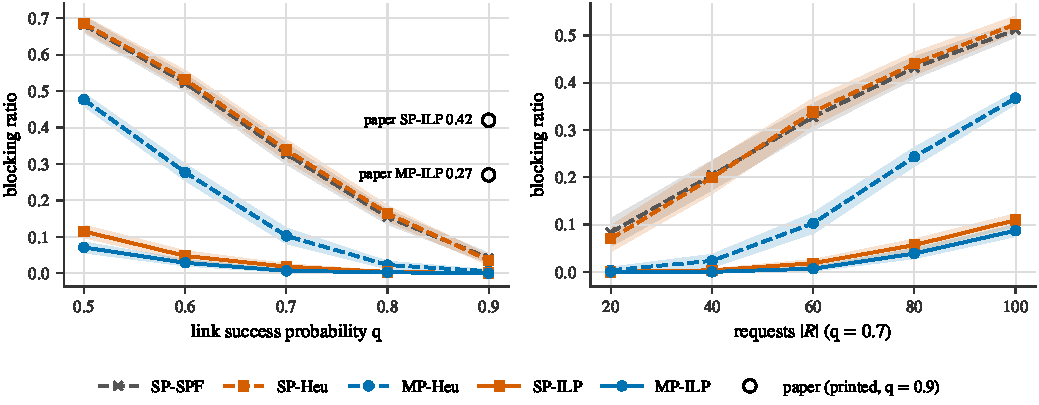
\includegraphics[width=\textwidth]{F1_partA_blocking.pdf}
\caption{Blocking ratio, mean and 95\% CI over 30 paired seeds. Left: against link success probability $q$, with the two values the paper prints for $q=0.9$. Right: against the number of requests at $q=0.7$. ILP solid, heuristic dashed.}
\label{fig:f1}
\end{figure*}

\subsection{What reproduced}
Multipath blocks fewer requests than single path, for the heuristics and for the ILPs, at every $q$ (Fig.~\ref{fig:f1}, left). At $q=0.5$ the heuristics block \brMPHeuqFive{} with splitting and \brSPHeuqFive{} without, and the ILPs block \brMPILPqFive{} and \brSPILPqFive. The same holds at every load (Fig.~\ref{fig:f1}, right); at $|R|=100$, MP-Heu blocks \brMPHeuRHundred{} and SP-Heu \brSPHeuRHundred.

The other trends also match the paper. Blocking falls as $q$ rises and grows with load. The ILPs are slower than the heuristics, and MP-ILP is the slowest. MP-Heu splits fewer requests as $q$ rises (Fig.~\ref{fig:f2}), although this is weak evidence because $\Gamma$ was the calibration target. SP-SPF and SP-Heu are almost identical, which suggests that the heuristic's path choice matters much less than its ability to split.

\subsection{What did not reproduce}
The absolute levels did not reproduce. At $q=0.9$ the paper prints 0.27 for MP-ILP and 0.42 for SP-ILP. Our ILPs block \brMPILPqNine{} and \brSPILPqNine. Under the same printed parameters, our network carries much less load than the paper's. Section~\ref{sec:sens} tests two readings of the request model that could explain this.

The paper also calls the heuristic and the ILP comparable. Ours are far apart at low $q$, where MP-Heu blocks \brMPHeuqFive{} and MP-ILP \brMPILPqFive. Two diagnostics at $q=0.5$ show where the gap comes from. ILP-$\delta$, an optimal solver that must keep the heuristic's headroom, blocks \brMPILPDeltaqFive. The heuristic with $\delta=1$, still greedy but without headroom, blocks \brMPHeuDoneqFive. Greedy search and the headroom rule each cost little alone and much more together, so the headroom rule hurts the greedy placer far more than an optimal one. Our extension builds on this result.

The ILP's $\Gamma$ was held out from calibration. Ours falls from \gammaMPILPqFive{} to \gammaMPILPqNine{} over the range of $q$. The paper's falls from \paperGammaMPILPqFive{} to \paperGammaMPILPqNine. The ILP's objective counts served requests and ignores paths, so many optimal solutions differ only in how often they split. $\Gamma$ of an ILP therefore depends on which optimum the solver returns, and the paper does not say how it chose.

Per run (all ten windows), our heuristics take under 0.1~s, our SP-ILP about \runtimeSPILPqFive~s, and our MP-ILP \runtimeMPILPqFive--\runtimeMPILPqEight~s. The paper reports \paperTimeSPILPqNine--\paperTimeSPILPqFive~s for SP-ILP and \paperTimeMPILPqNine--\paperTimeMPILPqFive~s for MP-ILP, with CPLEX. The order matches, with the heuristic fastest, then SP-ILP, then MP-ILP. Our times are far lower, but the solver, formulation and hardware all differ, so the times cannot be compared directly.

\begin{figure}[t]
\centering
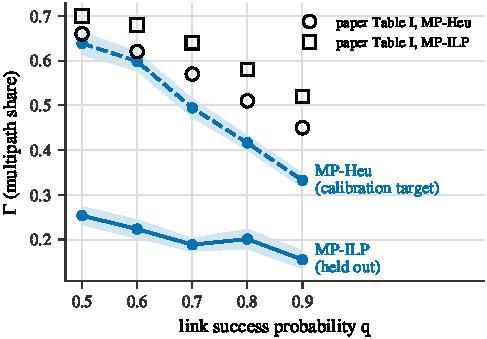
\includegraphics[width=\columnwidth]{F2_partA_gamma.pdf}
\caption{Share of served requests that used more than one path ($\Gamma$). MP-Heu was the calibration target. MP-ILP is held out. Open markers are the values in the paper's Table~I.}
\label{fig:f2}
\end{figure}

\begin{table}[t]
\caption{Values the paper prints, against ours}
\label{tab:paper}
\centering\small
\begin{tabular}{@{}lccl@{}}
\toprule
Quantity & Paper & Ours & Role \\
\midrule
BR, MP-ILP, $q=0.9$ & \paperBRMPILPqNine & \brMPILPqNine & held out \\
BR, SP-ILP, $q=0.9$ & \paperBRSPILPqNine & \brSPILPqNine & held out \\
$\Gamma$, MP-Heu, $q=0.5$ & \paperGammaMPHeuqFive & \gammaMPHeuqFive & calibrated \\
$\Gamma$, MP-Heu, $q=0.9$ & \paperGammaMPHeuqNine & \gammaMPHeuqNine & calibrated \\
$\Gamma$, MP-ILP, $q=0.5$ & \paperGammaMPILPqFive & \gammaMPILPqFive & held out \\
$\Gamma$, MP-ILP, $q=0.9$ & \paperGammaMPILPqNine & \gammaMPILPqNine & held out \\
Time (s), SP-ILP, $q=0.5$ & \paperTimeSPILPqFive & \runtimeSPILPqFive & other solver \\
Time (s), MP-ILP, $q=0.5$ & \paperTimeMPILPqFive & \runtimeMPILPqFive & other solver \\
\bottomrule
\end{tabular}
\end{table}

\subsection{Why are our blocking levels lower?}\label{sec:sens}
\begin{figure*}[t]
\centering
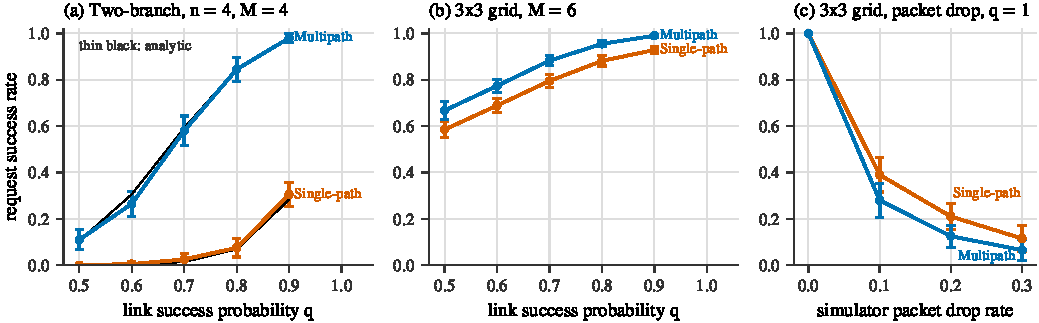
\includegraphics[width=\textwidth]{F3_partB_success.pdf}
\caption{Part B in QuNetSim: request success rate, mean and 95\% CI over 20 seeds. (a) Two-branch network with the exact binomial prediction (thin black). (b) $3\times3$ grid with four requests per window competing for the same links. (c) The grid under the simulator's own packet drop, with $q=1$ so that loss is the only cause of failure.}
\label{fig:f3}
\end{figure*}
Two other readings of the request model would load the network more. In the first (gaps, A3), the Poisson draws are gaps between arrivals rather than arrival slots. Arrivals then drift late, and requests that cannot finish before $T$ never enter the network; we count them as blocked. In the second (per slot, A27), a request needs $n$ pairs in each of its $h$ slots, or $nh$ pairs in its window. After Part A was frozen, we reran the four methods under each reading and under both together, with the same \sensSeeds{} seeds (Table~\ref{tab:sens}).

The per-slot reading comes close to the paper's levels. At $q=0.9$, MP-ILP blocks \sensBRPerSlotMPILPqNine{} and SP-ILP \sensBRPerSlotSPILPqNine, against the paper's \paperBRMPILPqNine{} and \paperBRSPILPqNine, with a similar gap between them. The gaps reading does not. It lifts every method to about the same level at $q=0.9$ (MP-ILP \sensBRGapsMPILPqNine, SP-ILP \sensBRGapsSPILPqNine), because the extra blocked requests never arrive before $T$ and no routing can serve them.

The per-slot reading is therefore the more plausible explanation of the level gap, though we cannot confirm it without the authors' code. Under every reading, multipath blocks no more than single path on average at both $q$ values tested. Even under the per-slot reading, our heuristic stays far from our ILP (MP-Heu \sensBRPerSlotMPHeuqNine{} at $q=0.9$), and that gap remains unexplained. Our headline results keep the reading we fixed before seeing any blocking ratio.

\begin{table}[t]
\caption{Blocking ratio at $q=0.9$ under other readings of the request model (\sensSeeds{} seeds, held out)}
\label{tab:sens}
\centering\small
\begin{tabular}{@{}lccc@{}}
\toprule
Reading & SP-ILP & MP-ILP & MP-Heu \\
\midrule
Ours (per window, direct arrivals) & \brSPILPqNine & \brMPILPqNine & \brMPHeuqNine \\
Gaps & \sensBRGapsSPILPqNine & \sensBRGapsMPILPqNine & \sensBRGapsMPHeuqNine \\
Per slot & \sensBRPerSlotSPILPqNine & \sensBRPerSlotMPILPqNine & \sensBRPerSlotMPHeuqNine \\
Gaps and per slot & \sensBRGapsPerSlotSPILPqNine & \sensBRGapsPerSlotMPILPqNine & \sensBRGapsPerSlotMPHeuqNine \\
Paper (printed) & \paperBRSPILPqNine & \paperBRMPILPqNine & n/a \\
\bottomrule
\end{tabular}
\end{table}

\section{Part B: QuNetSim Check}
\begin{figure*}[t]
\centering
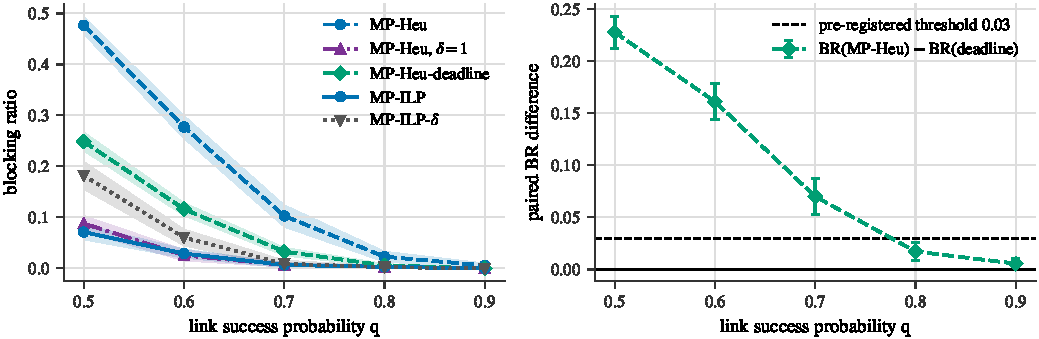
\includegraphics[width=\textwidth]{F4_partC_extension.pdf}
\caption{Extension. Left: blocking ratio against $q$ for the heuristic with $\delta=2$ (the paper), $\delta=1$ and deadline-aware $\delta$, with MP-ILP and ILP-$\delta$ for reference. Right: paired difference BR(MP-Heu) $-$ BR(deadline-aware) with 95\% CI. The dashed line is the pre-registered threshold.}
\label{fig:f4}
\end{figure*}
\subsection{Setup}
We use QuNetSim 0.1.3 on three networks: a chain A--B--C as a sanity check, a two-branch network with routes S--a1--a2--D and S--b1--b2--D, and a $3\times3$ grid. Every end-to-end pair is built hop by hop with QuNetSim calls. \texttt{send\_epr} creates a pair on each link, each middle node makes a Bell measurement and sends two classical bits to the destination, and the destination applies the X and Z corrections. Both ends then measure in Z or X. All \pbCorrelated{} of the \pbDelivered{} delivered pairs gave matching outcomes.

QuNetSim's per-link loss model never affects EPR pairs, its global packet drop rate also discards classical messages and acknowledgements, and injecting a failure inside its swap crashed it. We therefore give each link $M$ attempts per window, each landing with probability $q$ (A22). The attempts are shared by every request and path that uses the link, so multipath gets no extra attempts, only more of the network.

Single path uses QuNetSim's default router (a shortest path). Multipath uses $k=2$ link-disjoint paths and splits the pairs evenly. Requests are served one after another, because concurrent sends between the same hosts mix up their qubits (QuNetSim issue 170). A request succeeds only if all $n$ pairs arrive before a link on their route runs out of attempts. Each setting uses \pbSeeds{} seeds, with the same dice for single path and multipath. Separately, we run the handout's loss sweep with the simulator's own drop rate (E4).


\subsection{Results}
On the chain at $q=1$ every request succeeds. On the chain and the two-branch network, success has a closed form: a link that must carry $m$ pairs needs at least $m$ landings in $M$ attempts, which is a binomial tail. In \pbAnalyticInside{} of \pbAnalyticTotal{} settings, the exact value lies inside the 95\% Wilson interval of the simulated rate (Fig.~\ref{fig:f3}a). With QuNetSim's built-in swap and our multipath routes installed as its router, \pbCrossOk{} of \pbCrossTotal{} pairs were correlated, so the library's swap agrees with ours.

When link capacity is short, multipath succeeds more often. On the two-branch network with $n=4$ at $q=0.9$, multipath serves \pbTwoBranchMPnFourqNine{} of requests and single path \pbTwoBranchSPnFourqNine. Paired by seed, multipath did better in \pbBetterTwo{} of \pbRunsTwo{} runs and worse in \pbWorseTwo; the rest were ties, mostly where both methods always succeeded or always failed. On the grid, competing requests shrink the margin. At $q=0.5$ the success rates are \pbThreeGridMPnVarqFive{} and \pbThreeGridSPnVarqFive, and multipath did better in \pbBetterThree{} of \pbRunsThree{} runs and worse in \pbWorseThree. A third path ($k=3$) adds nothing measurable (\pbThreeKGridMPnVarqFive{} at $q=0.5$). Multipath also costs more: it uses \pbattThreeGridMPnVarqFive{} attempts per request against \pbattThreeGridSPnVarqFive{} on the grid at $q=0.5$, and pairs on a path that fails part-way are wasted.

Packet loss does not favour multipath (Fig.~\ref{fig:f3}c). With $q=1$ and the simulator's drop rate at 0.1, single path succeeds in \pbFourGridSPnVardOne{} of grid requests and multipath in \pbFourGridMPnVardOne. Paired by seed over the three drop rates, multipath did worse in \pbWorseFourGrid{} of \pbRunsFourGrid{} grid runs and better in \pbBetterFourGrid. A likely reason, which we did not test separately: for half of the grid's node pairs the second disjoint path is two links longer, and every extra link adds packets that can be lost. On the two-branch network both routes have three links, so the two methods send the same packets and give identical results (\pbFourBranchMPnTwodOne{} at 0.1). Success falls far faster than the drop rate, probably because each pair needs several packets: the EPR halves, their acknowledgements and the correction bits. In our runs, multipath helped when link capacity was short and did not help when every packet risked loss.

\subsection{How Part B differs from Part A}
When capacity is the limit (E2, E3), the ranking matches Part A, but the numbers cannot be compared, for four reasons. In Part A the planner knows every link's capacity before it routes; in Part B the routes are fixed first, and a request can fail part-way after spending attempts. Part B has no ILP and no priority $\rho$, so requests are served in arrival order. A failed attempt is retried while the link has attempts left, so the budget works as a shared pool rather than a fixed number of seats. Finally, QuNetSim does not model fidelity for these pairs, so only the hop limit carries over.

\section{Extension: Deadline-Aware Headroom}
The heuristic always keeps headroom: one request may take at most half of a link's pairs ($\delta=2$). The ILP has no such rule. Our variant keeps the headroom except when a request is on its last chance ($\rho=1$), where it uses $\delta=1$. Whether this helps was uncertain in advance. Taking more pairs for one request can block requests placed after it in the same window.

We fixed the hypothesis and the decision rule in the scope note before any run. On the small setup at $q=0.5$, deadline-aware $\delta$ lowers MP-Heu's blocking ratio by at least 3 percentage points. The hypothesis counts as supported if the paired mean difference is at least \extThreshold{} and the lower bound of its 95\% CI is above zero. We also report $\delta=1$ for every request, which tells us whether the deadline condition is what matters.

The hypothesis is \extVerdict. At $q=0.5$, the paired difference is \extDiffqFive{} (95\% CI \extCIloqFive{} to \extCIhiqFive) over 30 seeds. Measured as a ratio of means, the variant closes \extGapDeadqFive{} of the gap between MP-Heu and MP-ILP (Fig.~\ref{fig:f4}).

Using $\delta=1$ for every request does better still, with a difference of \extDoneDiffqFive{} and \extGapDoneqFive{} of the gap closed. At every $q$, $\delta=1$ is at least as good as the deadline-aware rule. In this model, then, the gain comes from dropping headroom, and the deadline condition adds nothing. A likely reason, which we did not test separately, is that headroom saves pairs for requests placed later in the same window, while requests are placed in priority order and capacity resets every window, so the saved pairs mostly go unused. The supported hypothesis is therefore a weaker finding than it first appears. We would drop the headroom rule rather than relax it near deadlines, and this should be retested in a model where pairs survive across windows.


\section{Limitations}
The abstract model is a simplification. Swapping always succeeds, every pair is discarded at the end of its window, memories do not decay within a window, and fidelity enters only as a hop limit. Real repeaters violate all four.

The QuNetSim results are a qualitative check, not real hardware. QuNetSim models no noise, decoherence or timing for EPR pairs, link failure comes from our own attempt budget (A22), and fidelity is not measured. Part B shows only that the ranking of single path and multipath holds in a packet-level simulator with real Bell-state measurements when capacity is the limit. Under the simulator's packet drop, it reverses.

The results depend on the parameters we chose. The paper does not give the demand $n$, the number of paths $K$ or the exact arrival model. We calibrated $n$ on a single quantity, and another reading of the request model gives blocking levels close to the paper's (Section~\ref{sec:sens}).

The fidelity model is inferred. Werner-state swapping reproduces both hop limits the paper prints, but the paper never names its model. We ran only the paper's small setup.

\section*{AI-Use Statement}
We used Claude (Anthropic), through Claude Code, as a programming and writing assistant. It surveyed the QuNetSim source and related literature, drafted code, tests and documents to our specifications, ran experiments, and reviewed our work critically. Every assumption, result and figure was checked against tests or hand-worked answers before we used it. \texttt{AI\_LOG.md} lists each request and what we kept, changed or rejected. One rejected example is the first extension idea, which a review showed was true by construction. We take responsibility for all content and can explain every line.

\begin{thebibliography}{9}
\bibitem{halder2024} J.~Halder, E.~Matus, and G.~Fettweis, ``On the concurrent multipath entanglement distribution in quantum networks,'' in \emph{Proc. IEEE GLOBECOM}, 2024, pp.~2791--2796.
\bibitem{qunetsim} S.~DiAdamo, J.~N\"otzel, B.~Zanger, and M.~M.~Be\c{s}e, ``QuNetSim: A software framework for quantum networks,'' \emph{IEEE Trans. Quantum Eng.}, vol.~2, 2021.
\bibitem{halder2024sr} J.~Halder \emph{et al.}, ``Optimal routing and end-to-end entanglement distribution in quantum networks,'' \emph{Sci. Rep.}, vol.~14, 2024.
\bibitem{briegel1998} H.-J.~Briegel, W.~D\"ur, J.~I.~Cirac, and P.~Zoller, ``Quantum repeaters: The role of imperfect local operations in quantum communication,'' \emph{Phys. Rev. Lett.}, vol.~81, p.~5932, 1998.
\bibitem{highs} Q.~Huangfu and J.~A.~J.~Hall, ``Parallelizing the dual revised simplex method,'' \emph{Math. Prog. Comp.}, vol.~10, pp.~119--142, 2018.
\bibitem{pulp} S.~Mitchell, M.~O'Sullivan, and I.~Dunning, ``PuLP: A linear programming toolkit for Python,'' Univ. of Auckland, 2011.
\end{thebibliography}

\end{document}
